\documentclass{article}
\usepackage{float}
\usepackage{graphicx}
\usepackage{amsmath}

\begin{document}

\title{Gradient Descent}
\author{Ta Quang Minh}
\date{\today}
\maketitle

\section{Introduction}
Gradient Descent is a widely used optimization algorithm employed in machine learning and various other fields to minimize the cost or loss function of a model. It iteratively adjusts the parameters of a model in the direction of the steepest descent of the cost function gradient, aiming to find the local minimum. This report provides an overview of the Gradient Descent method, its variants, applications, advantages, and limitations.

\section{Algorithm Overview}
The Gradient Descent algorithm works by iteratively updating the parameters of a model in the opposite direction of the gradient of the cost function. The general update rule for parameter $\theta$ is given by:
\[
\theta = \theta - \alpha \nabla J(\theta)
\]
Where:
\begin{itemize}
    \item $\theta$ represents the model parameters.
    \item $\alpha$ is the learning rate, determining the size of the step taken in each iteration.
    \item $\nabla J(\theta)$ denotes the gradient of the cost function $J(\theta)$ with respect to $\theta$.
\end{itemize}

\section{Applications}
Gradient Descent is extensively used in parameter estimation and function optimization. It is specifically employed by various machine learning models, including:
\begin{itemize}
    \item Linear and logistic regression
    \item Neural network training
    \item Support vector machines
    \item Dimensionality reduction techniques like PCA and t-SNE
    \item Clustering algorithms such as K-means
\end{itemize}

\section{Implementation details}
In the context of machine learning, the first step of implementing gradient descent is to express the appropriate loss function that we want to minimize in terms of parameters of the model.

The next step is to find the way to calculate the gradient of the function. The gradient is a  a generalization of the derivative of a scalar-valued function to functions of multiple variables. It consists of multiple partial derivatives of that function. The value of each partial derivative can be calculated by finding explicit formula or by approximation means.

When implementing the algorithm, the user should be able to choose the appropriate step size and convergence criteria according to each specific situation. The step size, or learning rate is very important because it greatly affects the convergence speed and quality of the return value. Adaptive learning rate which can be changed dynamically when running can therefore improve the algorithm greatly.

\section{Testing on some functions}
\subsection{Example 1}

Consider the function $f(x) = x^2 - 4x + 5$. We can see that this function has the minimum of 1 at x = 2 

Using gradient descent, we can start with the initial value = 5. Let the learning rate be 0.05, and we run at most 1000 iterations, stopping where the change in the value of the function converge to $10^{-6}$

\begin{figure}[H]
    \centering
    \resizebox{\textwidth}{!}{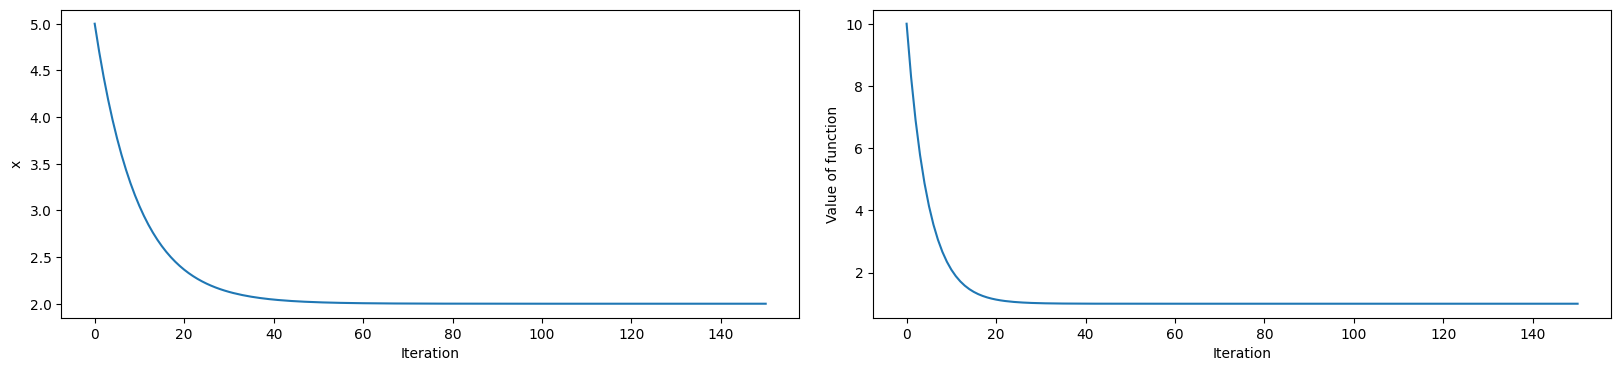
\includegraphics{assignment 1/grad_des1.png}}
    \caption{Value of x and of $f(x)$}
    \label{fig:example}
\end{figure}

The algorithm successfully looks for the argument x to minimize the function in 149 iterations. The approximate value for x is 2.00000046, and $f(x)$ is 1.0000000000002078 at this point.

If the step size is too high, for example I tried to take learning rate = 1.1, the algorithm keep oscillating and failed to converge.

\begin{figure}[H]
    \centering
    \resizebox{\textwidth}{!}{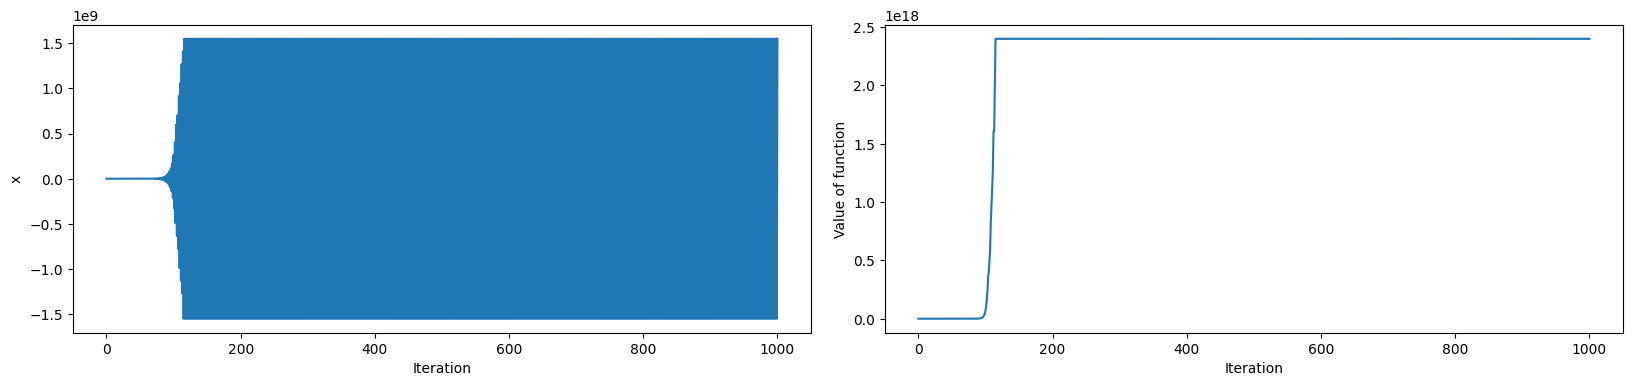
\includegraphics{assignment 1/grad_des3.png}}
    \caption{Value of x and of $f(x)$}
    \label{fig:example}
\end{figure}

\subsection{Example 2}
Consider the function $f(x,y) = x^2 + y^2$. We can see that this function has the minimum of 0 at x = y = 0.

Using gradient descent, we can start with the initial value = (4,4). Let the learning rate be 0.1, and we run at most 1000 iterations, stopping where the change in the value of the function converge to $10^{-6}$

\begin{figure}[H]
    \centering
    \resizebox{\textwidth}{!}{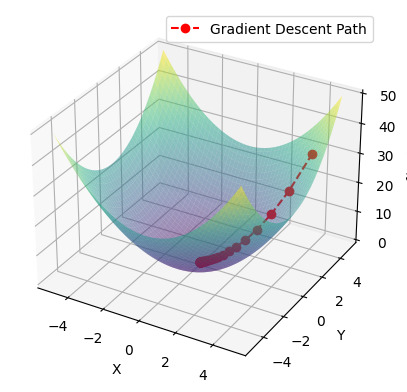
\includegraphics{assignment 1/grad_des2.png}}
    \caption{Value of x and of $f(x)$}
    \label{fig:example}
\end{figure}

The algorithm successfully looks for the argument x to minimize the function in 73 iterations.  The approximate value for (x,y) is (3.36999333e-07,3.36999333e-07), and $f(x,y)$ is 2.2713710127018717e-13 at this point. 

\section{Advantages}
\begin{enumerate}
    \item \textbf{Versatility:} Gradient Descent can be applied to a wide range of optimization problems, making it a versatile algorithm.
    \item \textbf{Scalability:} It can handle large datasets efficiently, especially with variants like SGD and mini-batch GD.
    \item \textbf{Convergence:} Under certain conditions, Gradient Descent guarantees convergence to a local minimum of the cost function.
\end{enumerate}

\section{Limitations}
\begin{enumerate}
    \item \textbf{Sensitivity to Learning Rate:} Choosing an appropriate learning rate is crucial for the convergence and performance of Gradient Descent. A too high or too low learning rate can lead to slow convergence or divergence.
    \item \textbf{Local Optima:} Gradient Descent may converge to a local minimum instead of the global minimum, depending on the initial parameters and the shape of the cost function.
    \item \textbf{Saddle Points:} In high-dimensional spaces, Gradient Descent may get stuck at saddle points, slowing down convergence.
\end{enumerate}

\section{Variants of Gradient Descent}
\begin{enumerate}
    \item \textbf{Batch Gradient Descent:} Computes the gradient of the cost function using the entire dataset in each iteration. It guarantees convergence to the global minimum but can be slow for large datasets.
    \item \textbf{Stochastic Gradient Descent (SGD):} Updates the parameters using only one random training sample at a time. It is computationally efficient but may exhibit high variance in the cost function.
    \item \textbf{Mini-batch Gradient Descent:} A compromise between Batch GD and SGD, where batches of fixed size are used to compute the gradient. It combines the advantages of both approaches.
    \item \textbf{Momentum Gradient Descent:} Introduces a momentum term to accelerate convergence and dampen oscillations in the parameter updates.
    \item \textbf{Adagrad, RMSprop, Adam:} Adaptive learning rate methods that adjust the learning rate for each parameter based on historical gradients, leading to faster convergence and better performance on non-convex optimization problems.
\end{enumerate}

\section{Conclusion}
Gradient Descent is a fundamental optimization algorithm widely used in machine learning and optimization tasks. Its variants and extensions have addressed many of its limitations, making it a powerful tool for training models and solving optimization problems in various domains. In this report, we have presented the theory, analysed the technique and applied the algorithm for concrete example.

Overall, understanding Gradient Descent and its variants is essential for practitioners in machine learning and optimization fields to effectively train models and achieve desired performance.

\end{document}
